\documentclass[a4paper,12pt]{article}

\usepackage{geometry}
\geometry{top=15mm}
\geometry{bottom=30mm}
\geometry{left=10mm}
\geometry{right=20mm}
\linespread{1}
\setlength{\parindent}{12pt}
\setlength{\parskip}{8pt}

\usepackage{titleps}

\newpagestyle{main}
{
  \setheadrule{0.4pt}
  \sethead{}{}{}
  \setfootrule{0,4pt}
  \setfoot{}{\thepage}{}
}
\usepackage{color}
\usepackage[english,russian]{babel}
\usepackage[T2A]{fontenc}
\usepackage[utf8]{inputenc}
\usepackage{amsthm,amsmath,amsfonts,amssymb,mathtools}
\usepackage{indentfirst}
\usepackage{lipsum}
\usepackage{graphicx}
\usepackage{float}
\usepackage{wrapfig}

\newcommand{\partdef}[2]{\frac{\partial \mathnormal{#1}}{\partial \mathnormal{#2}}}

\begin{document}
\textbf{Задача 1}
\newline
\begin{wrapfigure}{r}{0.6\textwidth}
    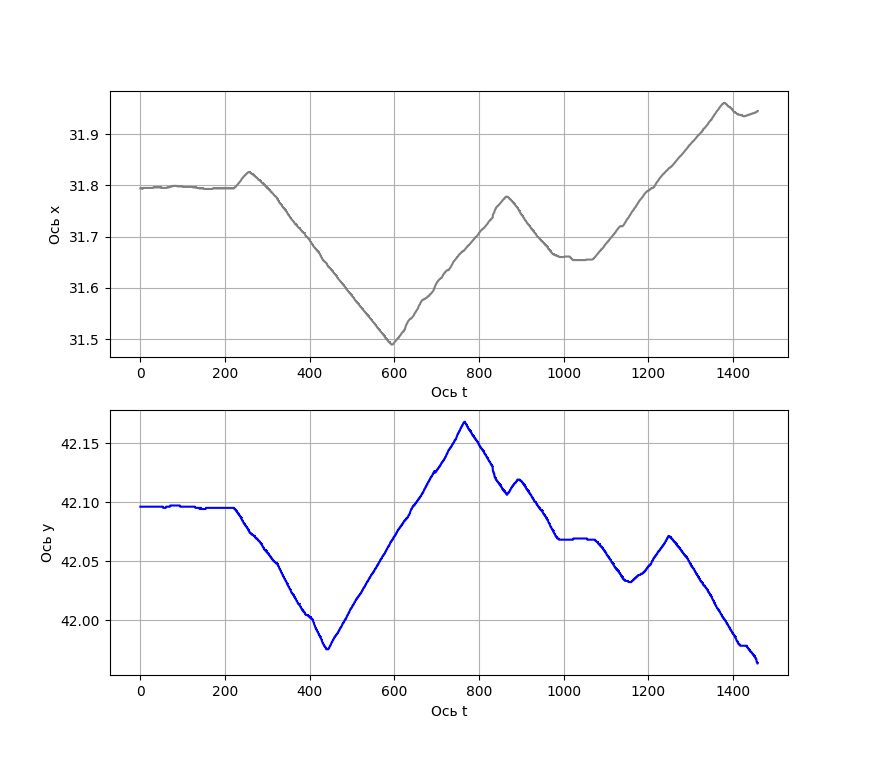
\includegraphics[width=0.6\textwidth]{Figure_1.png}
\end{wrapfigure}
УСЛОВИЕ:
\newline
Выбрать одну из сторон сквера и определить параметры
прямой методами- МНК, МНМ, РНК. Использование стандартного или
дифференциального режима - на ваше усмотрение.
\newline
РЕШЕНИЕ:
\newline
Будем использовать стандартный метод для исследования прямой. Нарисуем зависимость координат от времени. Понятно, что участку прямой будет соответствовать участок на графиках, где одновременна имеется и не нарушается монотонность. Таким образом находим нас интересующий участок.
\newline
\begin{figure}[H]
    \center{
        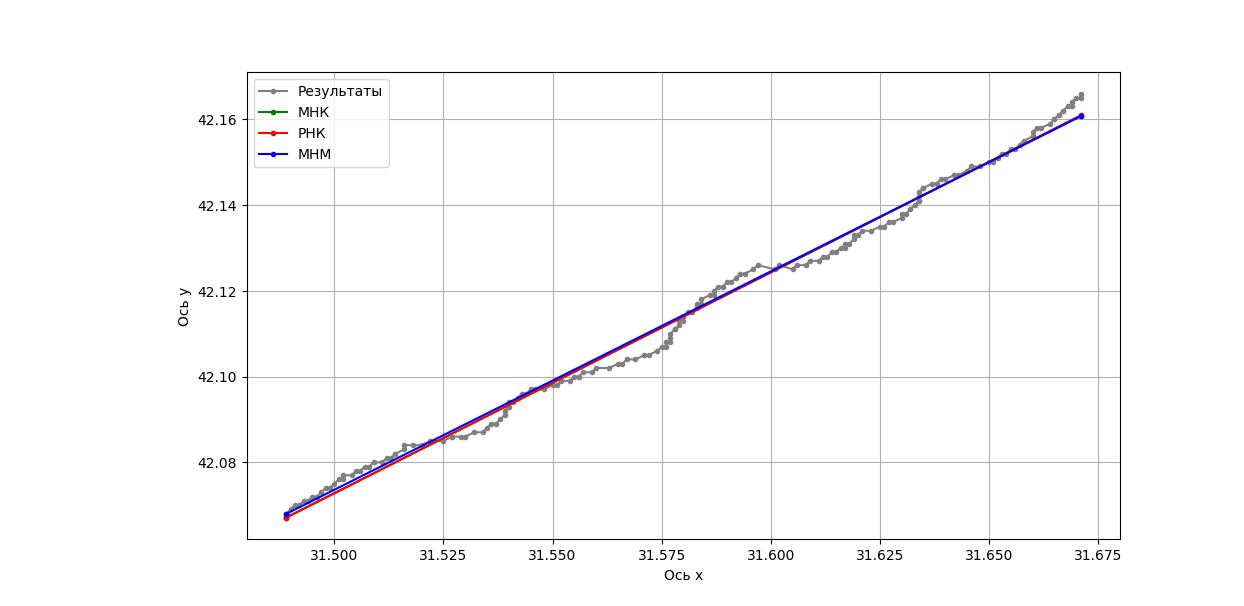
\includegraphics[width=1\linewidth]{Figure_2.png}
        }
\end{figure}
Выделяя участок и производя вычисления соответсвенными методами, имеем:
\newline
МНК $a_1 = -0.51468926 , a_2 = -25.86010734 \newline$
РНК $a_1 = -0.51536334 , a_2 = -25.83881892 \newline$
МНМ $a_1 = -0.50931677 , a_2 = -26.03012422 \newline$
    
ВОПРОСЫ:

\textit{1. Какие из погрешностей заметны в спутниковых данных и на каких участках траекторий?}
    
В день, когда мы делали работу шёл снег и было облачно. Поэтому на
протяжении всей работы наблюдается влияние атмосферы и затенение. 
Во время хождения по прямоугольнику мы находились под деревьми -
в связи с этим появляется многолучевость.

\textit{2. Сравните результаты, полученные тремя методами. Насколько отличаются оценки коэффициента наклона прямой в зависимости от метода обработки?}

Выше описаны результаты, которые были получены с помощью стандартного метода для нахаждения коэффициентов прямой. Угол находим по формуле: $\alpha = - \arctan a_1 $.
Поэтому получили следующий ряд результатов, которые удобно представить в виде таблицы:

\begin{align*}
    \begin{tabular}{|c|c|c|c|}
        \hline
        a_1,rad & a_1,^{\circ} &a_1,' &a_1,'' \\
        \hline   
        -0.4753298424487384 & -27.234393848931074 & -1634.0636309358645 & -98043.81785615187 \\
        \hline
        -0.47586260672201747 & -27.26491899326532 & -1635.895139595919 & -98153.70837575514 \\
        \hline
        -0.4710732150903613 & -26.990507066336146 & -1619.4304239801688 & -97165.82543881013 \\
        \hline
    \end{tabular}
\end{align*}

\textit{3. Оцените точность измерений приемников. }

Для решения этого пункта воспользуемся соотношением, полученном в алгоритме для поиска погрешности для прямой, $-\delta X = X_{1}^{'} a_{1} + X_{2}^{'} + 1_{N} a_{2}$. Так по нашему массиву данных с уже найденными коэффициентами $a_1$ и $a_2$ строим массив $\{\delta X\}$, и уже к этому массиву применяем алгоритм поиска среднеквадратичного отклонения. Получим следующие значения:
\newline
МНК:  $0.0010391160568508813$\newline
РНК:  $0.0010356346537859582$\newline
МНМ:  $0.0011573478344658367$\newline

\textit{4. В каком случае оценка коэффициента наклона прямой будет точнее – при использовании
дифференциального режима или стандартного? }

\begin{wrapfigure}{r}{0.6\textwidth}
    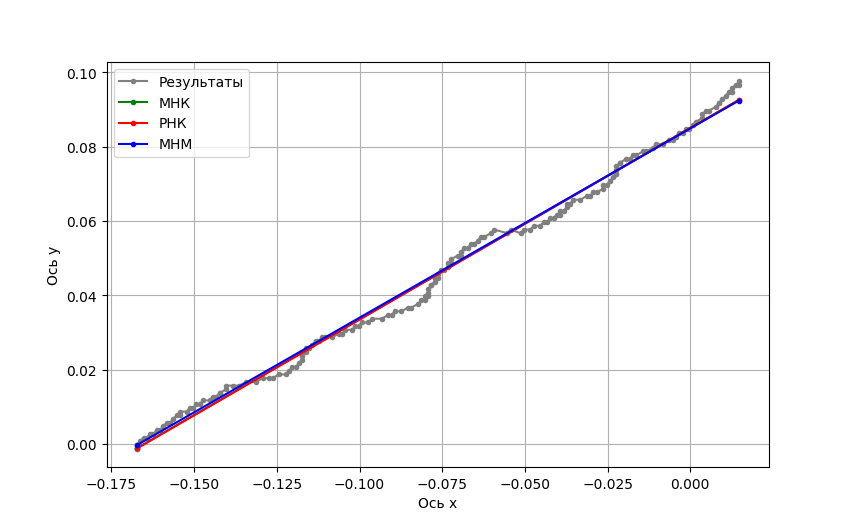
\includegraphics[width=0.6\textwidth]{Figure_5.png}
\end{wrapfigure}
Из задачи 2 возьмем координаты базы. Считаем необходимый участок первого ровера, и сосзадим массивы $\{x_{1}(t_{i})-x_{1}^{B}\}$ и $\{x_{2}(t_{i})-x_{2}^{B}\}$ , после чего применим к ним теже алгоритмы, что и при решении самой задачи 1. Получим следующие данные:
\newline
МНК:  $0.0010391160568510817$\newline
РНК:  $0.0010356346537858327$\newline
МНМ:  $0.0011573478345259555$\newline

Как видим, особого различия в точности измерений нет,как и предполагалось теорией, так как и в том, и в том случае погрешность оценки определяется инструментальной погрешностью.

\textbf{Задача 2}
Для решения дальнейших подзадач задачи 1, решим задачу 2 для нахождения координат базы.
Определить центр и радиус окружности (двумя методами – МНК, МНМ).\newline
\begin{wrapfigure}{r}{0.6\textwidth}
    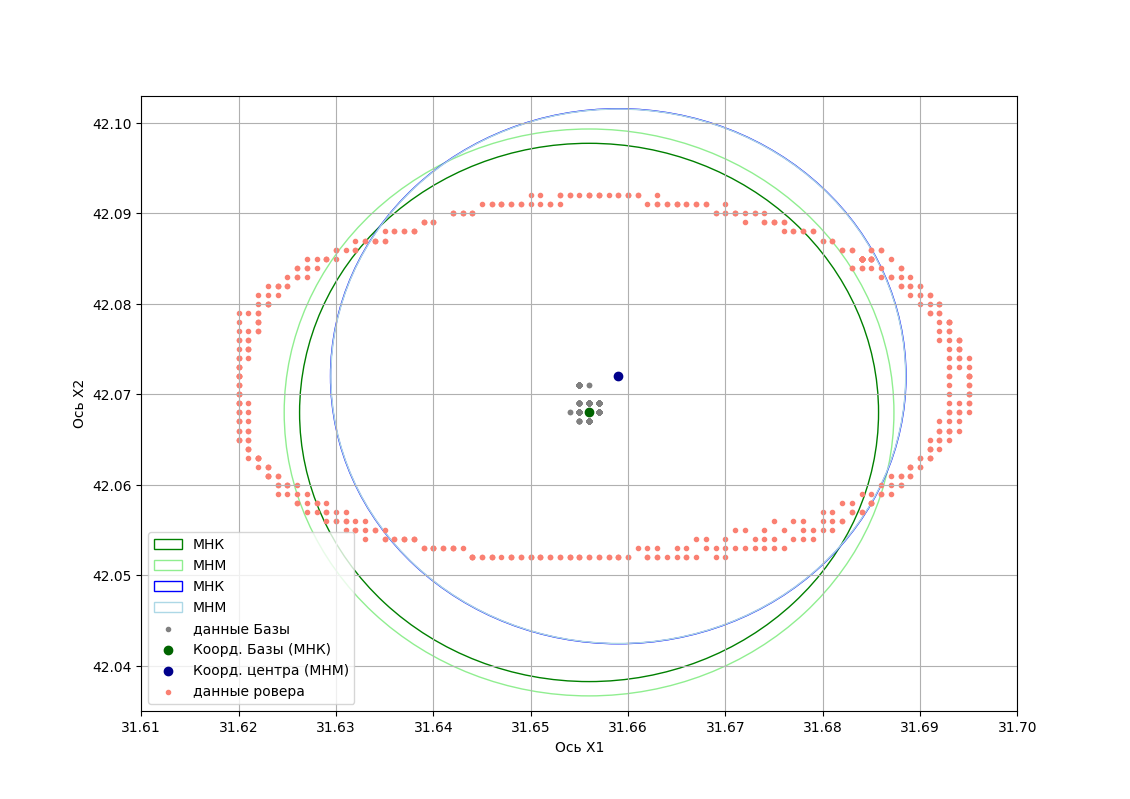
\includegraphics[width=0.6\textwidth]{Figure_4.png}
\end{wrapfigure}
Можем, как и выше описывалось, изобразить графики зависимости координат базы от времени и с помощью их определить промежуток, на котором хранятся необходимые данные(сделано за кадром). Используя даные базы, можем с помощью методов МНК и МНМ найти координаты базы и считать их центром нашей охружности. Тогда, используя данные ровера 2, создаем массив данных $r(t_i)=\sqrt{(x_1(t_i)-x_1^B)^2+(x_2(t_i)-x_2^B)^2}$ , и по этим данным с помошью МНК и МНМ получаем приближенное значение радиуса.
\newline
Можно пойти иным путем, записать данные ровера и найти центр окружности так: берем медианное значение по данным от каждой координаты по отдельности, полученная пара чисел - центр окружности. Затем можем создать аналогичный массив данных, как и выше, и произвести аналогичные вычисления.
\newline
$( 31.65630736842105 , 42.06826210526315 )$ - координаты базы по МНК.\newline
$( 31.656 , 42.068 )$ - координаты базы по МНМ.\newline
$( 31.659 , 42.072 )$ - координаты центра по МНМ.\newline
$0.029739726645681575$ - радиус по МНК (центр = база). \newline
$0.031320919526732834$ - радиус по МНМ (центр = база). \newline
$0.0295587434531364$ - радиус по МНМ (центр $\neq$ база).\newline
$0.029529646120468$ - радиус по МНМ (центр $\neq$ база).\newline

\end{document}